\documentclass[11pt]{amsart}
\usepackage[margin=1.15in]{geometry}
\usepackage{amssymb,mathtools}
\usepackage{tikz}
\usetikzlibrary{arrows.meta,positioning,calc,decorations.markings}
\usepackage[hidelinks]{hyperref}
\usepackage{url}

\newtheorem{theorem}{Theorem}
\newtheorem{proposition}[theorem]{Proposition}
\newtheorem{lemma}[theorem]{Lemma}
\newtheorem{corollary}[theorem]{Corollary}
\theoremstyle{definition}
\newtheorem{definition}[theorem]{Definition}
\theoremstyle{remark}
\newtheorem{remark}[theorem]{Remark}
\numberwithin{equation}{section}

\newcommand{\R}{\operatorname{Re}}
\newcommand{\I}{\operatorname{Im}}
\newcommand{\e}{e}
\newcommand{\nint}[1]{\|#1\|}
\DeclareMathOperator{\gpf}{P}

\title{The P\'olya--Vinogradov Inequality with $\log\log q$}
\author{Deep Bhattacharjee}
\date{21 November 2026}
\subjclass[2020]{Primary 11L40; Secondary 11M06, 11N36}
\keywords{character sums, P\'olya--Vinogradov inequality, Dirichlet $L$-functions}



\begin{document}
\sloppy
\begin{abstract}
Every primitive Dirichlet character $\chi$ modulo $q\ge3$ satisfies
$\bigl|\sum_{n\le x}\chi(n)\bigr|\le C\sqrt q\log\log q$ for all $x$, with an
absolute constant $C$, as soon as no Dirichlet $L$-function of a nonprincipal
character vanishes in the half-plane $\R s>7/8$. The generalized Riemann
hypothesis therefore gives the bound of Montgomery and Vaughan, and the
machine-checked half-plane of OpenAI gives it with no hypothesis. The bound
is sharp up to the constant. The whole argument is checked in Lean~4.
\end{abstract}
\maketitle

\section{Introduction}

For a nonprincipal Dirichlet character $\chi$ modulo $q$ put
\[
M(\chi)=\max_{x\ge1}\Bigl|\sum_{n\le x}\chi(n)\Bigr| .
\]
P\'olya~\cite{polya18} and Vinogradov~\cite{vinogradov18} proved in 1918 that
$M(\chi)\ll\sqrt q\log q$. Paley~\cite{paley32} showed that $M(\chi)\gg\sqrt
q\log\log q$ for infinitely many quadratic characters, and Montgomery and
Vaughan~\cite{mv77} proved under the generalized Riemann hypothesis that
$M(\chi)\ll\sqrt q\log\log q$ for every nonprincipal $\chi$. Between these two
results the order of $M(\chi)$ is determined up to the constant.\footnote{Later
work determines the constant for characters of a fixed odd order under the
generalized Riemann hypothesis and improves the unconditional bound
$\sqrt q\log q$ for those characters by a power of $\log q$; see Granville and
Soundararajan~\cite{gs07}, Goldmakher~\cite{goldmakher12} and Lamzouri and
Mangerel~\cite{lm22}. Those refinements use the structure of characters of
small order. The argument below treats every primitive character in the same
way and does not determine the constant.}

This paper proves the following.

\begin{definition}\label{def:H}
For $1/2\le\theta<1$ let $\mathrm H(\theta)$ be the statement that
$L(s,\xi)\ne0$ whenever $\xi$ is a nonprincipal Dirichlet character, of any
modulus, and $\R s>\theta$.
\end{definition}

The generalized Riemann hypothesis for Dirichlet $L$-functions is
$\mathrm H(1/2)$, and $\mathrm H(\theta)$ implies $\mathrm H(\theta')$ for
$\theta\le\theta'$.

\begin{theorem}\label{thm:main}
Assume $\mathrm H(7/8)$. There is an absolute constant $C$ such that every
primitive Dirichlet character $\chi$ modulo $q\ge3$ satisfies
\[
\Bigl|\sum_{n\le x}\chi(n)\Bigr|\le C\sqrt q\,\log\log q\qquad(x\ge1).
\]
\end{theorem}

\begin{corollary}[Montgomery--Vaughan]\label{cor:grh}
Under the generalized Riemann hypothesis the conclusion of
Theorem~\textup{\ref{thm:main}} holds.
\end{corollary}

\begin{corollary}\label{cor:uncond}
The conclusion of Theorem~\textup{\ref{thm:main}} holds without any
hypothesis.
\end{corollary}

Corollary~\ref{cor:uncond} rests on the theorem that $\mathrm H(7/8)$ holds.
That theorem was announced by OpenAI in October 2026 together with a proof
written in Lean~4 over Mathlib~\cite{openai}. We have compiled that proof,
all 2,924 of its files, together with our own, and the Lean kernel accepts
Corollary~\ref{cor:uncond} with only the three standard axioms of Lean
(Section~\ref{sec:lean}).\footnote{A kernel check establishes that the
formal statement follows from the axioms of Lean's type theory together with
\texttt{propext}, \texttt{Classical.choice} and \texttt{Quot.sound}. The formal
statement is
\texttt{OAI.DirichletCharacter.LFunction\_ne\_zero\_of\_seven\_eighths\_lt\_re},
which is phrased with Mathlib's own \texttt{DirichletCharacter.LFunction}, so it
says exactly that $L(s,\chi)\ne0$ for $\R s>7/8$ and every Dirichlet character
$\chi$, except at the pole $s=1$ of the principal character. No human-readable
proof of the half-plane $7/8$ has yet been refereed.}

The same method gives the range in which a character sum is small compared
with its length.

\begin{theorem}\label{thm:range}
Assume $\mathrm H(7/8)$. There is an absolute constant $C$ such that every
nonprincipal character $\chi$ modulo $q\ge3$ and every $x\ge2$ satisfy
\[
\Bigl|\sum_{n\le x}\chi(n)\Bigr|\le Cx\Bigl(\frac{\log\log q}{\log x}+\frac1{\log
q}\Bigr).
\]
\end{theorem}

In particular $\sum_{n\le x}\chi(n)=o(x)$ as soon as $\log x/\log\log
q\to\infty$, and Theorem~\ref{thm:range} holds under the generalized Riemann
hypothesis and, by the half-plane of~\cite{openai}, unconditionally.

\subsection*{The idea}

The argument is that of Montgomery and Vaughan~\cite{mv77}, and its point is
that it uses the zeros only through a zero-free half-plane to the right of
some $\theta<1$, never on the critical line. Pólya's Fourier expansion
(Section~\ref{sec:polya}) reduces $M(\chi)$ to the sums
\[
F_H(\beta)=\sum_{m\le H}\frac{\chi(m)\e(m\beta)}m,\qquad\e(x)=\e^{2\pi ix},
\]
with $H\le q$. Split $m$ according to its largest prime factor $\gpf(m)$. The
integers with $\gpf(m)\le Y$ contribute at most $\prod_{p\le Y}(1-1/p)^{-1}\ll\log
Y$, and the choice $Y=(\log q)^{700}$ makes this $O(\log\log q)$. For the
integers with a large prime factor, approximate $\beta$ by a fraction $a/r$.
If $r$ is large, the estimate of Montgomery and Vaughan for exponential sums
with multiplicative coefficients makes the sum small. If $r$ is small, the
additive character $\e(ma/r)$ is a combination of multiplicative characters
modulo $r$, and the sum becomes a combination of prime sums
$\sum_p\chi\psi(p)\e(p\gamma)$; the half-plane $\mathrm H(7/8)$ makes each of
these $O(x^{19/20})$, which beats the trivial bound by a power of the length.
Figure~\ref{fig:arcs} shows the dissection.

\begin{figure}[t]
\centering
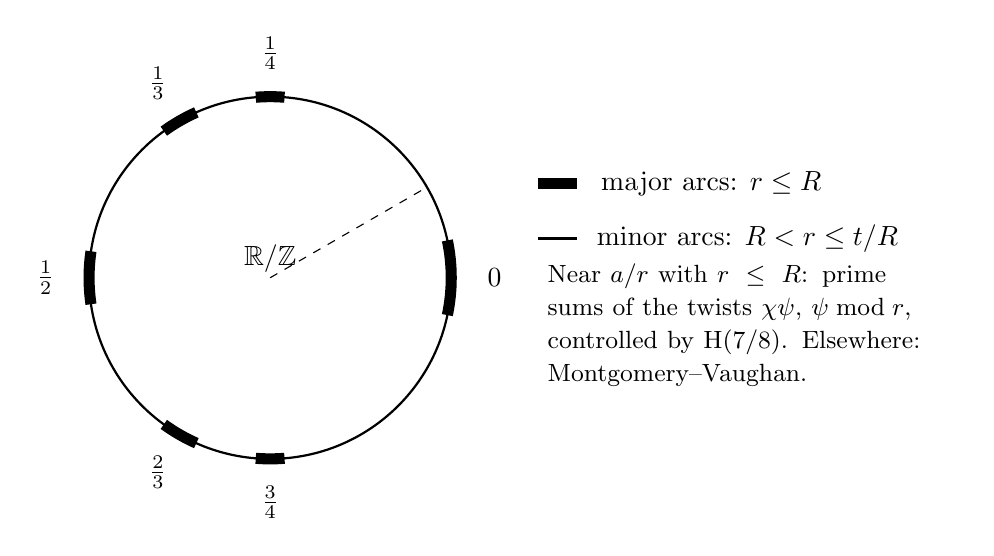
\begin{tikzpicture}[scale=1.0]
\draw[thick] (0,0) circle (2.3);
\foreach \a/\r in {0/0.34,180/0.24,120/0.17,240/0.17,90/0.13,270/0.13}{
  \draw[line width=4pt,black] (\a-\r*35:2.3) arc (\a-\r*35:\a+\r*35:2.3);
}
\foreach \a/\lab in {0/{$0$},180/{$\tfrac12$},120/{$\tfrac13$},240/{$\tfrac23$},90/{$\tfrac14$},270/{$\tfrac34$}}{
  \fill (\a:2.3) circle (1.5pt);
  \node at (\a:2.85) {\lab};
}
\draw[dashed] (0,0) -- (30:2.3);
\node at (0,0.25) {$\mathbb R/\mathbb Z$};
\draw[line width=4pt] (3.4,1.2) -- (3.9,1.2) node[right] {\ major arcs: $r\le R$};
\draw[thick] (3.4,0.5) -- (3.9,0.5) node[right] {\ minor arcs: $R<r\le t/R$};
\node[right,text width=5.2cm] at (3.4,-0.6) {\small Near $a/r$ with $r\le R$: prime sums of the twists $\chi\psi$, $\psi\bmod r$, controlled by $\mathrm H(7/8)$. Elsewhere: Montgomery--Vaughan.};
\end{tikzpicture}
\caption{The dissection of $\mathbb R/\mathbb Z$ used for the partial sums
$\mathcal A(t)=\sum_{n\le t,\ \gpf(n)>Y}\chi(n)\e(n\beta)$, drawn with a small
value of $R$. By Dirichlet's theorem every $\beta$ has an approximation
$|\beta-a/r|\le1/(r(Q+1))$ with $r\le Q=\lfloor t/R\rfloor$. The thick arcs are
the points with $r\le R$; their width at $a/r$ is of order $R/(rt)$. In the
proof $R=\lceil\log q\rceil^{16}$ and $Y=\lceil\log q\rceil^{700}$.}
\label{fig:arcs}
\end{figure}

\subsection*{Formal verification}

Every step of the proof, from the analytic properties of $L(s,\chi)$ that
Mathlib provides to the final inequality, is checked in Lean~4~\cite{lean4}
over Mathlib~\cite{mathlib20}. The sources are in the repository~\cite{repo}.
Theorem~\ref{thm:main} under $\mathrm H(7/8)$, Corollary~\ref{cor:grh} and
Theorem~\ref{thm:range} have their hypotheses as explicit arguments, and the
unconditional statements import the formal half-plane of~\cite{openai}. The
text below is a complete proof in ordinary mathematics; Section~\ref{sec:lean}
lists the formal names.

\subsection*{Notation}

Throughout, $p$ and $p'$ denote primes, $\Lambda$ is the von Mangoldt function,
$\e(x)=\e^{2\pi ix}$, and $\nint\theta$ is the distance from $\theta\in\mathbb
R$ to the nearest integer. For $n\ge2$, $\gpf(n)$ is the largest prime factor
of $n$, and $\gpf(1)=0$. We write $\Psi(x,Y)$ for the number of $n\le x$ with
$\gpf(n)\le Y$. A character is a Dirichlet character, and $\chi_0$ is the
principal one. The letters $C,C_1,C_2,\dots$ denote positive absolute
constants, not always the same at each occurrence, and $A\ll B$ means $|A|\le
CB$. Sums over $n\le x$ run over integers $1\le n\le x$.

\section{Gauss sums and P\'olya's expansion}\label{sec:polya}

\begin{lemma}\label{lem:gauss}
Let $\chi$ be primitive modulo $q$ and $\tau(\chi)=\sum_{a\bmod
q}\chi(a)\e(a/q)$. Then $\sum_{a\bmod q}\chi(a)\e(an/q)=\bar\chi(n)\tau(\chi)$
for every integer $n$, and $|\tau(\chi)|=\sqrt q$.
\end{lemma}

\begin{proof}
If $(n,q)=1$, substitute $a\mapsto a\bar n$. If $d=(n,q)>1$, put $q_1=q/d$.
Since $\chi$ is primitive it is not induced from a character modulo $q_1$, so
there is $c\equiv1\pmod{q_1}$, prime to $q$, with $\chi(c)\ne1$.\footnote{If
$\chi(c)=1$ for every $c$ prime to $q$ with $c\equiv1\pmod {q_1}$, then $\chi$
is constant on the cosets of the kernel of $(\mathbb Z/q)^\times\to(\mathbb
Z/q_1)^\times$, hence factors through a character modulo $q_1<q$; that is the
definition of an imprimitive character.} Then $cn\equiv n\pmod q$, and the
substitution $a\mapsto ca$ multiplies the sum by $\bar\chi(c)$ and leaves it
unchanged, so the sum vanishes, as does $\bar\chi(n)$. For the modulus,
Parseval's identity for the additive characters modulo $q$ gives
\[
\sum_{n\bmod q}\Bigl|\sum_{a}\chi(a)\e\Bigl(\frac{an}q\Bigr)\Bigr|^2=q\sum_a|\chi(a)|^2=q\varphi(q),
\]
while the left side is $|\tau(\chi)|^2\sum_n|\chi(n)|^2=\varphi(q)|\tau(\chi)|^2$
by the first part.
\end{proof}

\begin{lemma}\label{lem:geom}
For $0<|\vartheta|\le1/2$,
\[
\Bigl|\frac1{1-\e(-\vartheta)}-\frac1{2\pi i\vartheta}\Bigr|\le3 .
\]
\end{lemma}

\begin{proof}
With $y=\pi\vartheta$ one has $1-\e(-\vartheta)=2i\sin(y)\e^{-iy}$, so
$1/(1-\e(-\vartheta))=\frac12+\frac i2\cot y$. The difference in question is
$\frac12+\frac i2(\cot y-1/y)$, and the odd function $\cot y-1/y$ is
decreasing on $(0,\pi/2]$ with limit $0$ at $0$, so its modulus is at most
$2/\pi$ there. Hence the left side is at most $(\frac14+\frac1{\pi^2})^{1/2}<1$.
\end{proof}

\begin{proposition}[P\'olya's expansion]\label{prop:polya}
Let $\chi$ be primitive modulo $q\ge2$ and $B\ge0$, and suppose that
\[
\Bigl|\sum_{m\le H}\frac{\bar\chi(m)\e(m\beta)}m\Bigr|\le B\qquad\text{for
every }\beta\in\mathbb R\text{ and every integer }H\text{ with }2H\le q.
\]
Then $|\sum_{n\le T}\chi(n)|\le\sqrt q\,(B+6)$ for every $T\ge1$.
\end{proposition}

\begin{proof}
We may take $T$ to be an integer. By Lemma~\ref{lem:gauss} applied to $\bar\chi$,
$\chi(n)\tau(\bar\chi)=\sum_{a\bmod q}\bar\chi(a)\e(an/q)$. Represent the
residues by $-q/2<a\le q/2$; the term $a=0$ vanishes. Summing the geometric
series,
\[
\tau(\bar\chi)\sum_{n\le T}\chi(n)=\sum_{0<|a|\le q/2}\bar\chi(a)\bigl(\e(aT/q)-1\bigr)\frac1{1-\e(-a/q)} .
\]
Write $1/(1-\e(-a/q))=q/(2\pi ia)+\varrho(a)$ with $|\varrho(a)|\le3$
(Lemma~\ref{lem:geom}). The terms with $\varrho$ contribute at most $q\cdot2\cdot3=6q$.
The remaining terms, with $a=m$ and $a=-m$, are
\[
\frac q{2\pi i}\Bigl(\sum_{m\le H_+}\frac{\bar\chi(m)(\e(mT/q)-1)}m-\bar\chi(-1)\sum_{m\le H_-}\frac{\bar\chi(m)(\e(-mT/q)-1)}m\Bigr),
\]
where $H_+=\lfloor q/2\rfloor$ and $H_-=\lfloor(q-1)/2\rfloor$ both satisfy $2H\le
q$. These are four sums of the kind in the hypothesis, so they contribute at
most $4qB/(2\pi)\le qB$. Dividing by $|\tau(\bar\chi)|=\sqrt q$ gives the claim.
\end{proof}

So Theorem~\ref{thm:main} follows once $|F_H(\beta)|\ll\log\log q$ for the
primitive character $\bar\chi$, uniformly in $H\le q$ and $\beta$. This is
Theorem~\ref{thm:B} below.

\section{The analytic input}\label{sec:analytic}

This section derives, from $\mathrm H(7/8)$, a power saving for prime sums of
nonprincipal characters. It uses three properties of $L(s,\xi)$, proved here
from the series.

\begin{lemma}[Growth]\label{lem:growth}
Let $\xi$ be nonprincipal modulo $m$. Then $L(s,\xi)$ extends holomorphically
to $\R s>0$ and $|L(s,\xi)|\le m|s|/\R s$ there. In particular
$|L(s,\xi)|\le2m|s|$ for $\R s\ge1/2$.
\end{lemma}

\begin{proof}
Let $A(t)=\sum_{n\le t}\xi(n)$. Since the sum of $\xi$ over a full period is
$0$, $|A(t)|\le m$. Abel summation gives, for $\R s>1$,
$L(s,\xi)=s\int_1^\infty A(t)t^{-s-1}\,dt$. The integral converges absolutely
and locally uniformly in $\R s>0$, so it defines a holomorphic function there,
equal to $L(s,\xi)$ by uniqueness of analytic continuation, and its modulus is
at most $m|s|\int_1^\infty t^{-\sigma-1}dt=m|s|/\sigma$.
\end{proof}

\begin{lemma}[Euler logarithm]\label{lem:eulerlog}
For a character $\xi$ and $\R s>1$ put
$E_\xi(s)=-\sum_p\log(1-\xi(p)p^{-s})$, with the principal branch. Then $E_\xi$
is holomorphic on $\R s>1$, $\exp E_\xi(s)=L(s,\xi)$ there, and
$|E_\xi(s)|\le A_0:=1+2\sum_pp^{-3/2}$ for $\R s\ge3/2$, uniformly in $\xi$ and
in its modulus.
\end{lemma}

\begin{proof}
For $|z|\le1/2$ one has $|\log(1-z)|\le\sum_k|z|^k/k\le2|z|$. Each term is
holomorphic in $\R s>1$ and $|\xi(p)p^{-s}|\le p^{-\sigma}\le1/2$ there, so the
series is dominated on $\R s\ge\sigma_1>1$ by $2\sum_pp^{-\sigma_1}$, converges
locally uniformly, and its exponential is the Euler product of $L(s,\xi)$.
The bound follows with $\sigma_1=3/2$.
\end{proof}

The third property is a quantitative form of the principle that a holomorphic
function without zeros, of polynomial growth, has a small logarithm. It
combines the Borel--Carath\'eodory inequality with Hadamard's three circles
theorem~\cite[\S\S5.3, 5.5]{titchmarsh39}.

\begin{lemma}[Logarithmic control]\label{lem:logcontrol}
Let $0<\eta<1/1000$, $A\ge1$, $\mu\ge1$ and $\varepsilon>0$. There are
constants $D$ and $K$, depending only on $\eta,A,\mu,\varepsilon$, with the
following property. Let $1/2\le a\le1$, $\mathcal C\ge\e$, $c\in\mathbb C$, and let
$f$ be holomorphic and zero-free on the disc $|z-c|<2-a-2\eta$, with
$|f(z)|\le\mathcal C^\mu$ for $|z-c|<2-a-3\eta$. Suppose that on $|z-c|<1/2$ there
is a holomorphic $E$ with $\exp E=f$ and $|E|\le A$ on $|z-c|\le49/100$. Then
\begin{align*}
|f(z)|+|f(z)|^{-1}&\le D\,\mathcal C^{\varepsilon}&&(|z-c|\le2-a-6\eta),\\
|f'(z)/f(z)|&\le K\log\mathcal C&&(|z-c|\le2-a-8\eta).
\end{align*}
\end{lemma}

\begin{proof}
Put $\rho_0=2-a-2\eta$. On the simply connected disc $|z-c|<\rho_0$ the
zero-free $f$ has a holomorphic logarithm $g$; adding a multiple of $2\pi i$
we may take $g=E$ on $|z-c|<1/2$, since both are logarithms of $f$ there and
the disc is connected. Then $\R g=\log|f|\le\mu\log\mathcal C$ on
$|z-c|<\rho_1:=2-a-3\eta$, and $|g(c)|\le A$.

\emph{Step 1 (Borel--Carath\'eodory).} For $r<\rho_1$, the
Borel--Carath\'eodory inequality gives
\[
\max_{|z-c|=r}|g(z)-g(c)|\le\frac{2r}{\rho_1-r}\Bigl(\max_{|z-c|=\rho_1}\R g-\R g(c)\Bigr)\le\frac{2r}{\rho_1-r}(\mu\log\mathcal C+A).
\]
At $r=\rho_2:=2-a-4\eta$ the factor is $2\rho_2/\eta\le3/\eta$, so
$|g|\le K_1\log\mathcal C$ on $|z-c|\le\rho_2$ with $K_1=(3/\eta)(\mu+A)+A$,
using $\log\mathcal C\ge1$.

\emph{Step 2 (three circles).} The function $\log\max_{|z-c|=r}|g|$ is a
convex function of $\log r$. On $r_1=49/100$ the maximum is at most $A$, on
$r_3=\rho_2$ it is at most $K_1\log\mathcal C$, and $r_2=2-a-5\eta$ lies
strictly between them. With
$\lambda=\log(r_2/r_1)/\log(r_3/r_1)\in(0,1)$, convexity gives
$\max_{|z-c|=r_2}|g|\le A^{1-\lambda}(K_1\log\mathcal C)^{\lambda}$. Since
$r_3-r_2=\eta$ and $r_3\le3/2$, one has $1-\lambda\ge\lambda_0(\eta)>0$
uniformly in $a$, so $\lambda\le1-\lambda_0$.\footnote{Indeed
$r_2\le3/2$, so $\log(r_3/r_2)=\log(1+\eta/r_2)\ge\eta/(2r_2)\ge\eta/3$, while
$\log(r_3/r_1)\le\log(150/49)<2$, so
$1-\lambda=\log(r_3/r_2)/\log(r_3/r_1)\ge\eta/6$. The exponent $\lambda$
therefore stays below $1-\eta/6$ for every admissible $a$, and this uniformity
is what makes $D$ depend on $\eta$ only.} For $u\ge1$ and $0\le\lambda\le1-\lambda_0$
the function $u^\lambda$ is at most $\varepsilon u+D_1$ with $D_1$ depending
only on $\lambda_0,\varepsilon$ and $A,K_1$ (Young's inequality). Hence
$|g|\le\varepsilon\log\mathcal C+\log D$ on $|z-c|\le r_2$, by the maximum
principle on the whole disc. Exponentiating, $|f|=\e^{\R g}$ and $|f|^{-1}=\e^{-\R g}$
are each at most $D\mathcal C^\varepsilon$ on $|z-c|\le r_2$, which contains
$|z-c|\le2-a-6\eta$.

\emph{Step 3 (Cauchy).} By Step~1 $|g|\le K_1\log\mathcal C$ on $|z-c|\le\rho_2$,
and Cauchy's estimate on circles of radius $2\eta$ about points of
$|z-c|\le2-a-8\eta$ gives $|f'/f|=|g'|\le K_1\log\mathcal C/(2\eta)$ there.
\end{proof}

\begin{proposition}\label{prop:logderiv}
Let $0<\eta<1/1000$. There is $K=K(\eta)$ such that the following holds. Let $\xi$
be nonprincipal modulo $m$ and $1/2\le a\le1$, and suppose that $L(z,\xi)\ne0$ for
$\R z>a+2\eta$. Then for $a+8\eta\le\sigma\le2$ and real $t$,
\[
\Bigl|\frac{L'}L(\sigma+it,\xi)\Bigr|\le K\log\bigl(2m(3+|t|)^2\bigr).
\]
\end{proposition}

\begin{proof}
Apply Lemma~\ref{lem:logcontrol} with $f=L(\cdot,\xi)$, $c=2+it$, $\mu=1$,
$\mathcal C=2m(3+|t|)^2\ge\e$, and $E=E_\xi$ with $A=A_0$
(Lemma~\ref{lem:eulerlog}; the disc $|z-c|<1/2$ lies in $\R z>3/2$). The disc
$|z-c|<2-a-2\eta$ lies in $\R z>a+2\eta$, where $L$ has no zeros, and it lies in
$\R z>0$, where $L$ is holomorphic. On $|z-c|<2-a-3\eta$ one has $\R z\ge1/2$ and
$|z|\le4+|t|$, so Lemma~\ref{lem:growth} gives $|L(z,\xi)|\le2m(4+|t|)\le\mathcal C$.
Every point $\sigma+it$ with $a+8\eta\le\sigma\le2$ lies in $|z-c|\le2-a-8\eta$.
\end{proof}

\subsection{Riesz means}

For $a:\mathbb N\to\mathbb C$ and $x>0$ put
\[
R_a(x)=\sum_{n\le x}a(n)\Bigl(1-\frac nx\Bigr).
\]

\begin{lemma}\label{lem:riesz}
If $\sum_na(n)n^{-\sigma}$ converges absolutely for some $\sigma\ge1$, then
\[
R_a(x)=\frac1{2\pi i}\int_{\sigma-i\infty}^{\sigma+i\infty}\Bigl(\sum_n\frac{a(n)}{n^s}\Bigr)\frac{x^s}{s(s+1)}\,ds .
\]
\end{lemma}

\begin{proof}
The function $k(y)=\max(1-y,0)$ has Mellin transform $\int_0^1(1-y)y^{s-1}dy=1/(s(s+1))$
for $\R s>0$, and since $|1/(s(s+1))|\le2/(1+t^2)$ on $\R s\ge1$ the Mellin
inversion formula holds at every $y>0$: $k(y)=\frac1{2\pi i}\int_{(\sigma)}y^{-s}\frac{ds}{s(s+1)}$.
Apply it with $y=n/x$, multiply by $a(n)$ and sum; the interchange is justified
by $\sum_n|a(n)|n^{-\sigma}\int(1+t^2)^{-1}dt<\infty$.
\end{proof}

\begin{lemma}[Contour shift]\label{lem:shift}
Let $\alpha\le\beta$, $\kappa>1$, and let $h$ be holomorphic on a neighbourhood of the strip
$\alpha\le\R z\le\beta$, with $|h(\sigma+it)|\le C_h(1+|t|)^{-\kappa}$ there. Then
$\int_{\mathbb R}h(\alpha+it)\,dt=\int_{\mathbb R}h(\beta+it)\,dt$.
\end{lemma}

\begin{proof}
By Cauchy's theorem the integral of $h$ over the boundary of the rectangle
$\alpha\le\R z\le\beta$, $|\I z|\le T$ is $0$. The horizontal sides contribute at
most $2(\beta-\alpha)C_h(1+T)^{-\kappa}\to0$, and the vertical integrals converge
absolutely.\footnote{The formal proof covers a more general situation, in
which $h$ is only assumed to grow at most like $\exp(A|t|)$ in the strip and to
be integrable on the two lines; it inserts the regulator $\exp(\epsilon z^2)$,
which decays like $\exp(-\epsilon t^2)$, applies the case above, and lets
$\epsilon\to0$ by dominated convergence. We need only the special case stated.}
\end{proof}

\begin{proposition}[Riesz-weighted prime sums]\label{prop:rieszprime}
Let $0<\eta<1/1000$. There is $K'=K'(\eta)$ such that, if $\xi$ is
nonprincipal modulo $m$, $1/2\le a\le1$, and $L(z,\xi)\ne0$ for $\R z>a+2\eta$,
then for $x\ge1$
\[
\bigl|R_{\xi\Lambda}(x)\bigr|\le K'x^{a+8\eta}\log(m+2).
\]
\end{proposition}

\begin{proof}
The Dirichlet series of $\xi\Lambda$ is $-L'/L(s,\xi)$, absolutely convergent on
$\R s=2$. By Lemma~\ref{lem:riesz},
$R_{\xi\Lambda}(x)=\frac1{2\pi}\int_{\mathbb R}h(2+it)\,dt$ with
$h(z)=x^z(-L'/L)(z,\xi)/(z(z+1))$. Put $\sigma_0=a+8\eta$. On the strip
$\sigma_0\le\R z\le2$ the function $h$ is holomorphic, because $L(\cdot,\xi)$ is
holomorphic and zero-free there (Lemma~\ref{lem:growth} and the hypothesis).
By Proposition~\ref{prop:logderiv} and the elementary inequalities
\[
\log\bigl(2m(3+|t|)^2\bigr)\le10\log(m+2)(1+|t|)^{1/2},\qquad|z(z+1)|\ge\tfrac18(1+|t|)^2\quad(\R z\ge\tfrac12),
\]
one has $|h(\sigma+it)|\le80K\log(m+2)x^\sigma(1+|t|)^{-3/2}$ in the
strip.\footnote{For the first inequality note $3+|t|\le3(1+|t|)$, so the left
side is at most $\log(18m)+2\log(1+|t|)$, and $\log(1+u)\le2u^{1/2}$ and
$\log(18m)\le 5\log(m+2)$. For the second, $|z|\ge\max(\frac12,|t|)$ and
$|z+1|\ge\max(\frac32,|t|)$.} Lemma~\ref{lem:shift} with $\kappa=3/2$ moves the line of
integration to $\R z=\sigma_0$, and
\[
|R_{\xi\Lambda}(x)|\le\frac{80K}{2\pi}\log(m+2)x^{\sigma_0}\int_{\mathbb R}(1+|t|)^{-3/2}dt=\frac{320K}{2\pi}x^{\sigma_0}\log(m+2).\qedhere
\]
\end{proof}

\subsection{Removing the weight}

\begin{lemma}\label{lem:unsmooth}
Let $|a(n)|\le B$ for $n\le x+h$, where $x,h>0$. Then
\[
h\Bigl|\sum_{n\le x}a(n)\Bigr|\le\bigl|(x+h)R_a(x+h)-xR_a(x)\bigr|+Bh(h+1).
\]
\end{lemma}

\begin{proof}
Since $yR_a(y)=\sum_{n\le y}a(n)(y-n)$,
\[
(x+h)R_a(x+h)-xR_a(x)=h\sum_{n\le x}a(n)+\sum_{x<n\le x+h}a(n)(x+h-n),
\]
and the last sum has at most $h+1$ terms, each of modulus at most $Bh$.
\end{proof}

\begin{proposition}[Prime sums]\label{prop:primesum}
Assume $\mathrm H(7/8)$. There is an absolute constant $C$ such that for every
nonprincipal $\xi$ modulo $m$ and every $x\ge1$
\[
\Bigl|\sum_{n\le x}\xi(n)\Lambda(n)\Bigr|\le Cx^{19/20}\log(m+2),\qquad
\Bigl|\sum_{p\le x}\xi(p)\log p\Bigr|\le Cx^{19/20}\log(m+2).
\]
\end{proposition}

\begin{proof}
Take $\eta=1/2000$ and $a=7/8-1/1000$, so that $a+2\eta=7/8$ and the hypothesis
of Proposition~\ref{prop:rieszprime} is $\mathrm H(7/8)$ for $\xi$; then
$\sigma_0=a+8\eta=7/8+3/1000$. Let $h=x^{47/50}\le x$. For $n\le x+h\le2x$,
$|\xi(n)\Lambda(n)|\le\log(2x)$. Lemma~\ref{lem:unsmooth} and
Proposition~\ref{prop:rieszprime} give
\[
\Bigl|\sum_{n\le x}\xi(n)\Lambda(n)\Bigr|\le\frac{2(2x)K'(2x)^{\sigma_0}\log(m+2)}h+\log(2x)(h+1).
\]
The first term is $\ll x^{1+\sigma_0-47/50}\log(m+2)=x^{0.938}\log(m+2)$. The second is
at most $2\log(2x)x^{47/50}\le200(2x)^{1/100}x^{47/50}\ll x^{19/20}$, using
$\log u\le100u^{1/100}$. Both are $\ll x^{19/20}\log(m+2)$. The difference between
the two sums in the statement is a sum over prime powers $p^k\le x$ with $k\ge2$,
of modulus at most $\sum_{2\le k\le\log_2x}\sum_{p\le x^{1/k}}\log p\le\sqrt
x\log4\log_2x\ll x^{19/20}$ by Chebyshev's bound (Lemma~\ref{lem:mertens}).
\end{proof}

\begin{remark}
Under the generalized Riemann hypothesis one may take any $a>1/2$ above and
obtain $x^{1/2+\delta}$; the exponent $19/20$ is simply a convenient number
larger than $7/8+3/1000$ and $47/50$, and nothing below depends on its value
except through the requirement that it be less than $1$.
\end{remark}

\section{Prime sums on major arcs}\label{sec:major}

\begin{lemma}[Twisted prime sums]\label{lem:twist}
Assume $\mathrm H(7/8)$. For nonprincipal $\xi$ modulo $m$, integers $2\le A\le B$
and real $\vartheta$,
\[
\Bigl|\sum_{A<p\le B}\xi(p)\e(p\vartheta)\Bigr|\le C\,\frac{B^{19/20}\log(m+2)\,(2+2\pi|\vartheta|B)}{\log A}.
\]
\end{lemma}

\begin{proof}
Write $\xi(p)\e(p\vartheta)=\xi(p)\log p\cdot g(p)$ with $g(u)=\e(u\vartheta)/\log u$.
The partial sums $\sum_{A<p\le n}\xi(p)\log p$, $A\le n\le B$, are at most
$2CB^{19/20}\log(m+2)$ by Proposition~\ref{prop:primesum}. By Abel's
inequality the sum is at most this bound times $|g(B)|+\sum_{A\le n<B}|g(n+1)-g(n)|$.
Now $|g(B)|\le1/\log A$, and
\[
|g(n+1)-g(n)|\le\frac{|\e((n+1)\vartheta)-\e(n\vartheta)|}{\log n}+\Bigl(\frac1{\log
n}-\frac1{\log(n+1)}\Bigr)\le\frac{2\pi|\vartheta|}{\log A}+\Bigl(\frac1{\log
n}-\frac1{\log(n+1)}\Bigr),
\]
whose sum over $A\le n<B$ is at most $(2\pi|\vartheta|B+1)/\log A$.
\end{proof}

\begin{lemma}\label{lem:twistprim}
Let $\chi$ be primitive modulo $q$, let $1\le r<q$ and let $\psi$ be a
character modulo $r$. Then the character $\chi\psi$ modulo $qr$ is nonprincipal.
\end{lemma}

\begin{proof}
Let $d=(q,r)$, so $d\le r<q$. If $n$ is prime to $q$ and $n\equiv1\pmod d$, the
Chinese remainder theorem gives $n'\equiv n\pmod q$ with $n'\equiv1\pmod r$, and
$n'$ is prime to $qr$. If $\chi\psi$ were principal, then
$\chi(n)=\chi(n')\psi(n')=1$ for all such $n$, so $\chi$ would be trivial on the
kernel of $(\mathbb Z/q)^\times\to(\mathbb Z/d)^\times$, hence induced from a
character modulo $d<q$. This contradicts primitivity.
\end{proof}

\begin{lemma}[Major arcs]\label{lem:majorprime}
Assume $\mathrm H(7/8)$. Let $\chi$ be primitive modulo $q$, $1\le r<q$, $c\in\mathbb
Z$, $\vartheta\in\mathbb R$, and let $A\le B$ be integers with $A\ge\max(2,r)$. Then
\[
\Bigl|\sum_{A<p\le B}\chi(p)\e\Bigl(\frac{pc}r\Bigr)\e(p\vartheta)\Bigr|\le
C\,\frac{r\,B^{19/20}\log(qr+2)(2+2\pi|\vartheta|B)}{\log A}.
\]
\end{lemma}

\begin{proof}
Every prime $p>A\ge r$ is prime to $r$. On the units of $\mathbb Z/r$ the
function $u\mapsto\e(uc/r)$ equals $\sum_{\psi\bmod r}w_\psi\psi(u)$ with
$w_\psi=\varphi(r)^{-1}\sum_{u}\bar\psi(u)\e(uc/r)$, so $|w_\psi|\le1$, by
orthogonality of characters. Hence the sum equals
$\sum_\psi w_\psi\sum_{A<p\le B}(\chi\psi)(p)\e(p\vartheta)$.\footnote{Here
$\chi\psi$ is the character modulo $qr$ with $(\chi\psi)(n)=\chi(n)\psi(n)$ for
$n$ prime to $qr$ and $0$ otherwise. For the primes in the sum the two
descriptions agree: $p$ is prime to $r$, and if $p\mid q$ both sides are $0$.}
By Lemma~\ref{lem:twistprim} each $\chi\psi$ is nonprincipal modulo $qr$, and
Lemma~\ref{lem:twist} applies to it. There are $\varphi(r)\le r$ characters $\psi$.
\end{proof}

\section{Integers with a large prime factor}\label{sec:nonsmooth}

\begin{lemma}\label{lem:gpfdecomp}
For every $f:\mathbb N\to\mathbb C$ and integers $Y,t\ge0$,
\[
\sum_{\substack{n\le t\\ \gpf(n)>Y}}f(n)=\sum_{m\le t}\ \sum_{\substack{\max(Y,\gpf(m)-1)<p\le t/m}}f(pm).
\]
\end{lemma}

\begin{proof}
An integer $n$ with $\gpf(n)>Y$ factors uniquely as $n=pm$ with $p=\gpf(n)$;
then $p>Y$, $p\ge\gpf(m)$ and $m\le t/p$. Conversely every pair $(p,m)$ on the
right gives $n=pm$ with $\gpf(n)=p>Y$.
\end{proof}

\begin{proposition}[Non-smooth part on a major arc]\label{prop:nsmajor}
Assume $\mathrm H(7/8)$. Let $\chi$ be primitive modulo $q$, $1\le r<q$,
$b\in\mathbb Z$, $\beta\in\mathbb R$, and $Y\ge\max(2,r)$, $t\ge1$ integers. Then
\[
\Bigl|\sum_{\substack{n\le t\\ \gpf(n)>Y}}\chi(n)\e\Bigl(n\Bigl(\frac br+\beta\Bigr)\Bigr)\Bigr|\le
C\,\frac{r\log(qr+2)(2+2\pi|\beta|t)}{Y^{1/20}\log Y}\,t .
\]
\end{proposition}

\begin{proof}
By Lemma~\ref{lem:gpfdecomp} and complete multiplicativity, the sum is
$\sum_m\chi(m)\sum_p\chi(p)\e(p\cdot mb/r)\e(p\cdot m\beta)$, where the inner
sum is over $A_m<p\le t/m$, $A_m=\max(Y,\gpf(m)-1)\ge\max(2,r)$, and is empty
unless $m<t/Y$. Lemma~\ref{lem:majorprime} with $c=mb$, $\vartheta=m\beta$ and
$B=\lfloor t/m\rfloor$ bounds the inner sum by
$C\,r(t/m)^{19/20}\log(qr+2)(2+2\pi|\beta|t)/\log Y$, since $|m\beta|B\le|\beta|t$.
Finally $\sum_{m\le t/Y}m^{-19/20}\le20(t/Y)^{1/20}$ and
$t^{19/20}(t/Y)^{1/20}=t\,Y^{-1/20}$.
\end{proof}

\section{Smooth numbers}\label{sec:smooth}

\begin{lemma}[Chebyshev and Mertens]\label{lem:mertens}
For every $n\ge1$ and $N\ge1$,
\[
\sum_{p\le n}\log p\le n\log4,\qquad\sum_{p\le n}\frac{\log p}p\le\log n+\log4,\qquad\sum_{p\le N}\frac1p\le\log\log N+10 .
\]
\end{lemma}

\begin{proof}
The first is Chebyshev's bound~\cite{chebyshev52}: the product of the primes
in $(m+1,2m+1]$ divides $\binom{2m+1}m\le4^m$, and induction on $n$ gives
$\prod_{p\le n}p\le4^n$. For the second~\cite{mertens74}, Legendre's formula
gives $v_p(n!)\ge\lfloor n/p\rfloor$, so
\[
n\log n\ge\log n!\ge\sum_{p\le n}\Bigl\lfloor\frac np\Bigr\rfloor\log p\ge n\sum_{p\le n}\frac{\log p}p-\sum_{p\le n}\log p,
\]
and the first bound finishes it. The third follows from the second by Abel
summation against $1/\log u$: with $S(u)=\sum_{p\le u}\log p/p\le\log u+\log4$,
\[
\sum_{p\le N}\frac1p=\frac{S(N)}{\log N}+\int_2^N\frac{S(u)}{u\log^2u}\,du\le
\Bigl(1+\frac{\log 4}{\log 2}\Bigr)+\bigl(\log\log N-\log\log2\bigr)+\frac{\log4}{\log2},
\]
which is at most $\log\log N+10$; for $N<3$ the statement is trivial.\footnote{The
formal proof uses the discrete form of Abel summation, with the weights
$1/\log n-1/\log(n+1)\le1/(n\log^2n)$, and obtains the same constant.}
\end{proof}

\begin{lemma}[Sums over smooth numbers]\label{lem:smooth}
For $Y\ge2$ and every $H$,
\[
\sum_{\substack{n\le H\\ \gpf(n)\le Y}}\frac1n\le\prod_{p\le Y}\Bigl(1-\frac1p\Bigr)^{-1}\le\e^{11}\log
Y .
\]
\end{lemma}

\begin{proof}
Expanding each factor in a geometric series shows that the product is the sum
of $1/n$ over all $n$ with $\gpf(n)\le Y$, which gives the first inequality.
For the second, $-\log(1-1/p)\le1/p+1/(p(p-1))$, and
$\sum_p1/(p(p-1))\le\sum_{k\ge2}1/(k(k-1))=1$, so the logarithm of the product is at
most $\log\log Y+11$ by Lemma~\ref{lem:mertens}.
\end{proof}

\begin{lemma}[Chebyshev's bound for $\Psi$]\label{lem:psi}
For integers $x\ge1$, $Y\ge1$,
\[
\Psi(x,Y)\log x\le x\bigl(1+2\log Y+2\log4\bigr).
\]
\end{lemma}

\begin{proof}
For $n\le x$, $\log x=\log(x/n)+\log n$. First,
$\sum_{n\le x}\log(x/n)=x\log x-\log x!\le x$. Second,
\[
\sum_{\substack{n\le x\\ \gpf(n)\le Y}}\log n=\sum_{\substack{n\le x\\ \gpf(n)\le Y}}\ \sum_{p\le Y}v_p(n)\log p\le\sum_{p\le
Y}\log p\sum_{n\le x}v_p(n)=\sum_{p\le Y}v_p(x!)\log p,
\]
and $v_p(x!)\le x/(p-1)\le2x/p$, so this is at most $2x(\log Y+\log 4)$ by
Lemma~\ref{lem:mertens}.
\end{proof}

\section{Exponential sums with multiplicative coefficients}\label{sec:mv}

This section proves a weak form of the estimate of Montgomery and
Vaughan~\cite[Corollary~1]{mv77}. Their bound has $(\log R)^{3/2}R^{-1/2}$ in place
of $(\log N)^2R^{-1/4}$ below; the weaker form suffices for
Theorem~\ref{thm:main} because $R$ will be a large power of $\log q$.

\begin{theorem}[Montgomery--Vaughan, weak form]\label{thm:mv}
There is an absolute constant $C$ with the following property. Let
$f:\mathbb N\to\mathbb C$ be completely multiplicative with $|f(n)|\le1$, let $a/r$
be a fraction in lowest terms and $\alpha$ real with $|\alpha-a/r|\le r^{-2}$, and
let $2\le R\le r\le N/R$. Then
\[
\Bigl|\sum_{n\le N}f(n)\e(n\alpha)\Bigr|\le C\Bigl(\frac N{\log N}+\frac{N(\log N)^2}{R^{1/4}}\Bigr).
\]
\end{theorem}

Write $S=\sum_{n\le N}f(n)\e(n\alpha)$, $w_M(\vartheta)=\min(M,1/\nint\vartheta)$
(with $w_M(\vartheta)=M$ when $\nint\vartheta<1/M$), and, for a prime $p$,
$T_p=\sum_{m\le N/p}f(m)\e(pm\alpha)$.

\subsection{Reduction to primes}

\begin{lemma}\label{lem:reduction}
$\bigl|S\log N-\sum_{p\le N}\log p\,f(p)\,T_p\bigr|\le CN$.
\end{lemma}

\begin{proof}
First, $|S\log N-\sum_{n\le N}f(n)\e(n\alpha)\log n|\le\sum_{n\le N}\log(N/n)\le N$.
Next, $\log n=\sum_{d\mid n}\Lambda(d)$, and, writing $n=dm$ and using
$f(dm)=f(d)f(m)$,
\[
\sum_{n\le N}f(n)\e(n\alpha)\log n=\sum_{d\le N}\Lambda(d)f(d)\sum_{m\le N/d}f(m)\e(dm\alpha).
\]
The terms with $d$ a prime are $\sum_p\log p\,f(p)T_p$. The others have
$d=p^k$, $k\ge2$, and contribute at most $N\sum_{p,k\ge2}\log p/p^k\le N\sum_p\log
p/(p(p-1))\ll N$.
\end{proof}

\subsection{Geometric sums and spacing}

\begin{lemma}\label{lem:spacing}
Let $|\alpha-a/r|\le r^{-2}$ with $r\ge2$ the denominator of $a/r$.
\begin{enumerate}
\item If $k\ne0$ is an integer with $2|k|\le r$, then $\nint{k\alpha}\ge1/(2r)$.
\item For $t\ge0$, the number of $1\le h\le H$ with $\nint{h\alpha}<t$ is at most
$(4H/r+1)(4rt+1)$.
\item For $M>0$ and $M\le2^K$, $\sum_{h\le H}w_M(h\alpha)\le(4H/r+1)(3M+4r+8rK)$.
\item For $M>0$, $\sum_{h\le H}w_M(h\alpha)^2\le(4H/r+1)(20rM+3M^2)$.
\end{enumerate}
\end{lemma}

\begin{proof}
(1) $\nint{ka/r}\ge1/r$ because $r\nmid ka$, while $|k\alpha-ka/r|\le|k|/r^2\le1/(2r)$.
(2) Let $L=\lfloor r/2\rfloor\ge r/4$ and split $[1,H]$ into at most
$H/L+1\le4H/r+1$ blocks of at most $L$ consecutive integers. Inside a block, two integers $h\ne h'$ have
$0<|h-h'|<L$, so by (1) the points $h\alpha$ and $h'\alpha$ are at distance at
least $1/(2r)$ modulo $1$. Points of the block with $\nint{h\alpha}<t$ lie, modulo
$1$, in an interval of length $2t$ and are $1/(2r)$-separated, so there are at
most $4rt+1$ of them.
(3) and (4) follow from (2) by the layer-cake decomposition: $w_M(\vartheta)\le M$
if $\nint\vartheta<1/M$, and if $2^{k-1}/M\le\nint\vartheta<2^k/M$ then
$w_M(\vartheta)\le M2^{1-k}$, so
\[
w_M(\vartheta)\le M\,\mathbf 1[\nint\vartheta<1/M]+\sum_{k=1}^K2M2^{-k}\mathbf 1[\nint\vartheta<2^k/M],
\]
and likewise with squares and $4M^24^{-k}$. Summing (2) against these weights
and using $\sum_k2^{-k}\le1$, $\sum_k4^{-k}\le1/3$ gives the bounds.\footnote{For
(3): $\sum_h w_M(h\alpha)\le(4H/r+1)\bigl(M(4r/M+1)+\sum_{k\le K}2M2^{-k}(4r2^k/M+1)\bigr)\le
(4H/r+1)(4r+M+8rK+2M)$. For (4) the layer sum is
$(4H/r+1)\bigl(M^2(4r/M+1)+\sum_k4M^24^{-k}(4r2^k/M+1)\bigr)\le(4H/r+1)(4rM+M^2+16rM+\tfrac43M^2)$.
In (4) the integer $K$ with $M\le2^K$ is chosen minimal, and the sum
$\sum_k2^{-k}$ is used.}
\end{proof}

\begin{lemma}[Bilinear sums]\label{lem:bilinear}
Let $A<B\le A+U$ be integers, $U>0$, let $V$ be a finite set of positive integers
and $b:V\to\mathbb C$. Then
\[
\sum_{A<u\le B}\Bigl|\sum_{\substack{v\in V\\ uv\le N}}b(v)\e(uv\alpha)\Bigr|^2\le\sum_{v,v'\in
V}|b(v)||b(v')|\,w_U\bigl((v-v')\alpha\bigr).
\]
Moreover $\sum_{m,m'\le H}w_M((m-m')\alpha)\le H\bigl(M+2\sum_{h\le H}w_M(h\alpha)\bigr)$.
\end{lemma}

\begin{proof}
Expanding the square, the left side is
$\sum_{v,v'}b(v)\bar b(v')\sum_u\e(u(v-v')\alpha)$, where $u$ runs over an
interval of at most $U$ integers. A geometric sum over $J$ consecutive integers
is at most $\min(J,1/(2\nint\vartheta))\le w_U(\vartheta)$. For the second
statement group the pairs by $h=|m-m'|$; each $h\ge1$ occurs at most $2H$ times,
and $h=0$ occurs $H$ times with weight $M$.
\end{proof}

\subsection{Small primes}

\begin{lemma}\label{lem:small}
Let $r\ge2$ and $J\ge1$. Then
\[
\Bigl|\sum_{p\le2^J}\log p\,f(p)T_p\Bigr|\le3\sqrt7\,J\sqrt{N2^J}+J^2N\sqrt{24/r}+896N+J^2\sqrt{24JNr}.
\]
\end{lemma}

\begin{proof}
Split the primes into blocks $U<p\le2U$, $U=2^j$, $j<J$. By Cauchy--Schwarz and
$\sum_{U<p\le2U}\log^2p\le U\log^2(2U)\le U(j+1)^2$,
\[
\Bigl|\sum_{U<p\le2U}\log p\,f(p)T_p\Bigr|^2\le U(j+1)^2\sum_{U<u\le2U}\Bigl|\sum_{m\le
H}\mathbf 1[um\le N]f(m)\e(um\alpha)\Bigr|^2,
\]
with $H=\lfloor N/U\rfloor$, where we extended the sum from primes to all
integers $u$ of the block. Lemma~\ref{lem:bilinear} bounds the inner sum by
$H(U+2\sum_{h\le H}w_U(h\alpha))$, and Lemma~\ref{lem:spacing}(3) with $M=U=2^j$ and $K=j$ by
\[
\frac NU\Bigl(U+2\Bigl(\frac{4N}{rU}+1\Bigr)\bigl(3U+4r+8rj\bigr)\Bigr)=7N+\frac{24N^2}{rU}+\frac{(32+64j)N^2}{U^2}+\frac{(8+16j)Nr}U,
\]
on expanding the product. Multiplying by
$U(j+1)^2$ and taking square roots with $\sqrt{a+b}\le\sqrt a+\sqrt b$, the block
contributes at most
$(j+1)\bigl(\sqrt{7NU}+N\sqrt{24/r}+N\sqrt{(32+64j)/U}+\sqrt{(8+16j)Nr}\bigr)$.
Sum over $j<J$: $\sum_j(j+1)\sqrt{2^j}\le3J\sqrt{2^J}$; $\sum_j(j+1)\le J^2$;
$\sqrt{(32+64j)/2^j}\le8(j+1)(3/4)^j$ and $\sum_j(j+1)^2(3/4)^j\le112$; and
$(8+16j)\le24J$.
\end{proof}

\subsection{Large primes and the pair sieve}

For the large primes the roles are reversed: the outer variable is $m$, which
is small, and the inner variable is the prime $p$. The bilinear lemma then
requires an upper bound for the number of prime pairs $p,p+h$, which is
supplied by Selberg's sieve.

\begin{proposition}[Prime pairs]\label{prop:pairs}
For $X\ge2$ and even $h\ne0$, with $G(h)=\prod_{p\mid h}p/(p-1)$,
\[
\#\{n<X:\ n\text{ and }n+h\text{ prime}\}\le\frac{400\,G(h)^2X}{\log^2X}+3X^{3/5}.
\]
\end{proposition}

\begin{proof}
Let $y=X^{1/5}$, $z=\lfloor y\rfloor$, let $\mathcal P$ be the product of the primes
$p\le z$ with $p\nmid h$, and sift the sequence $n(n+h)$, $n<X$, by the primes
dividing $\mathcal P$. A prime pair with $n>z$ survives, so the count is at most
$z+1$ plus the sifted number $S$. For $d\mid\mathcal P$, which is squarefree and
prime to $h$, the number of $n<X$ with $d\mid n(n+h)$ is $X\nu(d)+R_d$, where
$\nu$ is the completely multiplicative function with $\nu(p)=2/p$ and
$|R_d|\le\tau(d)$: for each factorisation $d=d_1d_2$ the conditions $d_1\mid n$,
$d_2\mid n+h$ define one residue class modulo $d$, by the Chinese remainder
theorem, and an interval of length $X$ meets it $X/d+O(1)$ times, with error at
most $1$. Selberg's upper bound sieve~\cite{selberg47},~\cite[Theorem~3.2]{hr74} gives
\[
S\le\frac X{\mathcal G}+\sum_{d\mid\mathcal P,\ d\le y}3^{\omega(d)}|R_d|,\qquad\mathcal G=\sum_{\substack{d\mid\mathcal
P\\ d\le\sqrt y}}\prod_{p\mid d}\frac{\nu(p)}{1-\nu(p)} .
\]
Every prime dividing $\mathcal P$ is at least $3$, because $h$ is even, so
$3^{\omega(d)}\le d$ and $|R_d|\le\tau(d)=2^{\omega(d)}\le d$; the error is at
most $\sum_{d\le y}d^2\le y^3=X^{3/5}$, and $z+1\le2X^{3/5}$. For the main term,
$\mathcal G$ is at least $\bigl(\sum_{m\le T,\ (m,h)=1}1/m\bigr)^2$ whenever
$T^2\le\sqrt y$.\footnote{Write $\nu(p)/(1-\nu(p))=\sum_{k\ge1}\nu(p)^k$; then
$\mathcal G$ is at least the sum of $\nu(m)=2^{\Omega(m)}/m$ over the integers
$m\le\sqrt y$ all of whose prime factors divide $\mathcal P$, and
$2^{\Omega(m)}\ge\#\{(m_1,m_2):m_1m_2=m\}$. The pairs with $m_1,m_2\le T$ give the
square. In the formal proof this is \texttt{Hs\_sq\_le\_boundingSum}.} Removing a
prime $p\mid h$ from a reciprocal sum costs at most the factor $p/(p-1)$, so
$\sum_{m\le T,\,(m,h)=1}1/m\ge\log(T+1)/G(h)$. Take $T=\lfloor X^{1/20}\rfloor$, so
that $T^2\le\sqrt y$ and $\log(T+1)\ge\frac1{20}\log X$. Then $\mathcal G\ge(\log
X)^2/(400G(h)^2)$, and the proposition follows.
\end{proof}

\begin{lemma}\label{lem:G4}
$\sum_{h\le X}G(h)^4\le\e^{30}X$.
\end{lemma}

\begin{proof}
$(p/(p-1))^4\le1+30/p$ for every prime, so $G(h)^4\le\sum_{S}\prod_{p\in S}30/p$ over
the sets $S$ of primes dividing $h$. The number of $h\le X$ divisible by
$\prod_{p\in S}p$ is at most $X/\prod_{p\in S}p$, so the sum is at most
$X\prod_p(1+30/p^2)\le X\exp(30\sum_pp^{-2})\le\e^{30}X$.
\end{proof}

\begin{lemma}\label{lem:W}
Let $V$ be a set of odd primes in $[1,X]$, $X\ge1$, $U>0$, and $|\alpha-a/r|\le r^{-2}$
with $r\ge2$. Then
\[
\sum_{p,p'\in V}w_U((p-p')\alpha)\le XU+\frac{800(X+1)}{\log^2(X+1)}\,\e^{15}\sqrt X\sqrt{(4X/r+1)(20rU+3U^2)}+6(X+1)^{3/5}XU .
\]
\end{lemma}

\begin{proof}
The diagonal gives at most $\#V\cdot U\le XU$. Off the diagonal group the pairs
by $h=|p-p'|\le X$; each $h$ contributes $2w_U(h\alpha)\#\{p\in V:p+h\in V\}$.
For odd $h$ this count is $0$, and for even $h$ it is at most
$400G(h)^2(X+1)/\log^2(X+1)+3(X+1)^{3/5}$ by Proposition~\ref{prop:pairs}. The first
part summed against $w_U(h\alpha)$ is bounded by Cauchy--Schwarz,
Lemma~\ref{lem:spacing}(4) and Lemma~\ref{lem:G4}; the second by $w_U\le U$.
\end{proof}

\begin{lemma}\label{lem:large}
Let $\ell=\lfloor\log_2N\rfloor\ge64$, $I=\lfloor\log_2\ell\rfloor+1$ and $J=\ell+1-4I$,
and let $2\le R\le r\le N/R$. Then
\[
\Bigl|\sum_{2^J<p\le N}\log p\,f(p)T_p\Bigr|\le
C\Bigl(N+\frac{IN}{R^{1/4}}+2^IN^{3/4}+4^I\log(N+1)\sqrt{N(2N)^{3/5}}\Bigr).
\]
\end{lemma}

\begin{proof}
Since $N<2^J16^I$, every $m\le N/p$ with $p>2^J$ lies in one of the blocks
$\mathcal B_i=[16^i,16^{i+1})$, $i<I$. Fix $i$, put $U=15\cdot16^i$ and $X=\lfloor
N/16^i\rfloor$; a prime $p$ with $pm\le N$ for some $m\in\mathcal B_i$ satisfies
$p\le X$, and $p>2^J\ge2$ is odd. By Cauchy--Schwarz over the at most $U$
integers $m\in\mathcal B_i$, then Lemma~\ref{lem:bilinear} with the roles of the
variables exchanged ($u=m$, $v=p$),
\[
\Bigl|\sum_p\log p\,f(p)\sum_{m\in\mathcal B_i,\ pm\le N}f(m)\e(pm\alpha)\Bigr|^2\le U\log^2(X+1)\sum_{p,p'\le
X}w_U((p-p')\alpha),
\]
where $V$ is the set of primes in $(2^J,X]$. Lemma~\ref{lem:W} bounds the right
side by three terms. The first, $XU$, contributes
$\sqrt{U\log^2(X+1)XU}=U\sqrt X\log(X+1)\le15\cdot4^i\sqrt N\log(N+1)$. The third
contributes $U\log(X+1)\sqrt{6(X+1)^{3/5}X}\ll4^i\log(N+1)\sqrt{N(2N)^{3/5}}$. In
the second the logarithms cancel, and with $X+1\le2X$ it is at most a constant
times $Z=UX^{3/2}\sqrt{(4X/r+1)(20rU+3U^2)}$. Expanding,
\[
\sqrt{(4X/r+1)(20rU+3U^2)}\le\sqrt{80XU}+\sqrt{12XU^2/r}+\sqrt{20rU}+\sqrt3\,U,
\]
so $\sqrt Z$ is at most a constant times
\[
U^{3/4}X+UXr^{-1/4}+(UX)^{3/4}r^{1/4}+UX^{3/4}.
\]
Since $UX\le15N$, $U\le15\cdot16^i$ and $R\le r\le N/R$, these four terms are
$\ll N2^{-i}$, $\ll N R^{-1/4}$, $\ll N^{3/4}(N/R)^{1/4}=NR^{-1/4}$ and
$\ll U^{1/4}(UX)^{3/4}\ll2^iN^{3/4}$.\footnote{The exact inequality, with the
constant $40$, is \texttt{sqrtZ\_le} in the formal proof.} Summing over $i<I$ with
$\sum_i2^{-i}\le2$, $\sum_i2^i\le2^I$, $\sum_i4^i\le4^I$ gives the lemma.
\end{proof}

\begin{proof}[Proof of Theorem~\textup{\ref{thm:mv}}]
If $\ell<64$, then $N<2^{65}$ and $|S|\le N\le65N/\log_2N$. Otherwise choose
$I,J$ as in Lemma~\ref{lem:large}; then $2^J\le N$, $J^2 2^J\le2N$, $4I\le\ell$,
$J\le\ell$ and $2^I\le2\ell$.\footnote{From $2^{I-1}\le\ell<2^I$ we get
$2^I\le2\ell$, and $J=\ell+1-4I\ge1$ because $4I\le4\log_2\ell+4\le\ell$ for $\ell\ge64$. Then
$J^22^J\le\ell^2 2^{\ell+1}/16^I\le2^{\ell+1}\le2N$, using $16^I\ge\ell^4\ge \ell^2$.} By
Lemma~\ref{lem:reduction},
\[
|S|\log N\le CN+\Bigl|\sum_{p\le2^J}\Bigr|+\Bigl|\sum_{2^J<p\le N}\Bigr| .
\]
In Lemma~\ref{lem:small}: $J\sqrt{N2^J}\le\sqrt2N$; $J^2N\sqrt{24/r}\ll N\log^2N/R^{1/2}$;
and $J^2\sqrt{24JNr}\ll(\log N)^{5/2}N/R^{1/2}$ since $r\le N/R$. In
Lemma~\ref{lem:large}: $I\le\log N$; $2^IN^{3/4}\le2\ell N^{3/4}\ll N$; and
$4^I\log(N+1)\sqrt{N(2N)^{3/5}}\le4\ell^2\log(N+1)\sqrt{N(2N)^{3/5}}\ll N$ because
$(\log x)^3\sqrt{x(2x)^{3/5}}\le2\cdot15^3x$. Altogether
$|S|\log N\ll N+N(\log N)^3R^{-1/4}$, which is the theorem.
\end{proof}

\section{The sums $F_H(\beta)$}\label{sec:B}

\begin{proposition}\label{prop:partial}
Assume $\mathrm H(7/8)$. There are absolute constants $C_1,C_2$ such that the
following holds. Let $\chi$ be primitive modulo $q$, let $2\le R<q$, let $Y\ge R$ and
$t>Y$ be integers, and $\beta$ real. Then $\mathcal A(t)=\sum_{n\le t,\
\gpf(n)>Y}\chi(n)\e(n\beta)$ satisfies
\[
|\mathcal A(t)|\le C_1\Bigl(\frac t{\log t}+\frac{t\log^2t}{R^{1/4}}\Bigr)+\Psi(t,Y)+C_2\,\frac{R\log(qR+2)(2+2\pi
R)}{Y^{1/20}\log Y}\,t .
\]
\end{proposition}

\begin{proof}
Put $Q=\lfloor t/R\rfloor\ge1$. By Dirichlet's approximation
theorem~\cite[Theorem~185]{hw08} there is a fraction $a/r$ in lowest terms with
$1\le r\le Q$ and $|\beta-a/r|\le1/(r(Q+1))$.

\emph{Minor arc, $r>R$.} Then $|\beta-a/r|\le1/r^2$ and $R<r\le Q\le t/R$, so
Theorem~\ref{thm:mv} with $f=\chi$ and $N=t$ bounds the complete sum
$\sum_{n\le t}\chi(n)\e(n\beta)$ by the first term. The terms with $\gpf(n)\le Y$
number $\Psi(t,Y)$ and each has modulus at most $1$.

\emph{Major arc, $r\le R$.} Then $r\le R<q$, $r\le Y$, and
$|\beta-a/r|\,t\le t/(r(Q+1))<R/r\le R$ since $Q+1>t/R$.
Proposition~\ref{prop:nsmajor} with $b=a$ and $\beta-a/r$ in place of $\beta$
gives at most
$C\,r\log(qr+2)(2+2\pi R)t/(Y^{1/20}\log Y)$, and $r\le R$.
\end{proof}

\begin{theorem}\label{thm:B}
Assume $\mathrm H(7/8)$. There is an absolute constant $C$ such that for every
primitive $\chi$ modulo $q$ with $\log q\ge200$, every integer $1\le H\le q$ and
every real $\beta$,
\[
\Bigl|\sum_{m\le H}\frac{\chi(m)\e(m\beta)}m\Bigr|\le C\log\log q .
\]
\end{theorem}

\begin{proof}
Let $L=\log q$, $M=\lceil L\rceil$, $R=M^{16}$ and $Y=M^{700}$. Then $2\le R\le Y$,
and $R<q$ because $16\log(L+1)<L$ for $L\ge200$. Split the sum according to
$\gpf(m)\le Y$ or $\gpf(m)>Y$. The first part is at most $\e^{11}\log Y\le
1400\e^{11}\log L$ by Lemma~\ref{lem:smooth}, since $\log Y=700\log M\le1400\log
L$.

For the second part, Abel summation with $\mathcal A(t)$ as above and
$w(t)=1/t-1/(t+1)$ gives
\[
\Bigl|\sum_{\substack{m\le H\\ \gpf(m)>Y}}\frac{\chi(m)\e(m\beta)}m\Bigr|\le1+\sum_{1\le t<H}|\mathcal A(t)|\,w(t),
\]
and $\mathcal A(t)=0$ for $t\le Y$. For $Y<t<H\le q$ apply
Proposition~\ref{prop:partial} and use $t\,w(t)\le1/t$, $\log t\le L$:
\begin{itemize}
\item $\sum_t\frac{t}{\log t}w(t)\le\sum_{t\le q}\frac1{t\log t}\le3+\log L$;
\item $\sum_t\frac{t\log^2t}{R^{1/4}}w(t)\le\frac{L^2}{M^4}\sum_{t\le q}\frac1t\le\frac{L^2(1+L)}{M^4}\le128$;
\item $\sum_t\Psi(t,Y)w(t)=\sum_{n<H,\ \gpf(n)\le Y}(1/n-1/H)\le\e^{11}\log Y$, since $n$ is counted for $n\le t<H$;
\item $\sum_t\kappa\,t\,w(t)\le\kappa(1+L)\le1$, where
$\kappa=R\log(qR+2)(2+2\pi R)/(Y^{1/20}\log Y)$, because $Y^{1/20}=M^{35}$ while the
numerator is at most $M^{16}\cdot3M\cdot8M^{16}$.
\end{itemize}
Altogether the sum is at most $2\cdot1400\e^{11}\log L+1+C_1(3+\log L+128)+C_2$,
which is $\ll\log L=\log\log q$.
\end{proof}

\section{Proofs of the theorems}\label{sec:proofs}

\begin{proof}[Proof of Theorem~\textup{\ref{thm:main}}]
The conjugate $\bar\chi$ is primitive modulo $q$. If $\log q\ge200$,
Theorem~\ref{thm:B} for $\bar\chi$ gives the hypothesis of
Proposition~\ref{prop:polya} with $B=C\log\log q$, hence $|\sum_{n\le
x}\chi(n)|\le\sqrt q(C\log\log q+6)\le(C+6)\sqrt q\log\log q$, since $\log\log
q\ge1$. If $\log q<200$, every sum $\sum_{m\le H}\bar\chi(m)\e(m\beta)/m$ is at most
$1+\log H<201$, and Proposition~\ref{prop:polya} gives $|\sum_{n\le x}\chi(n)|\le
207\sqrt q\le(207/\log\log3)\sqrt q\log\log q$.
\end{proof}

\begin{proof}[Proof of Corollaries~\textup{\ref{cor:grh}} and~\textup{\ref{cor:uncond}}]
The generalized Riemann hypothesis is $\mathrm H(1/2)$, which implies $\mathrm
H(7/8)$. For Corollary~\ref{cor:uncond}, $\mathrm H(7/8)$ is the theorem of~\cite{openai}.
\end{proof}

\begin{proof}[Proof of Theorem~\textup{\ref{thm:range}}]
Let $Y=\lceil\log q\rceil^{40}$ and $x\ge2$ an integer. The integers $n\le x$ with
$\gpf(n)>Y$ contribute, by Lemma~\ref{lem:gpfdecomp} and Lemma~\ref{lem:twist}
with $\vartheta=0$ applied to $\xi=\chi$ (no primitivity is needed when there is
no additive twist),
\[
\ll\sum_{m\le x/Y}\frac{(x/m)^{19/20}\log(q+2)}{\log Y}\ll\frac{x\log(q+2)}{Y^{1/20}\log Y}=\frac{x\log(q+2)}{\lceil\log
q\rceil^2\cdot40\log\lceil\log q\rceil}\ll\frac x{\log q}.
\]
The integers with $\gpf(n)\le Y$ number $\Psi(x,Y)\le x(1+2\log Y+2\log4)/\log
x\ll x\log\log q/\log x$ by Lemma~\ref{lem:psi}.
\end{proof}

\begin{remark}
The only property of the zeros used anywhere is $\mathrm H(7/8)$, through
Proposition~\ref{prop:primesum}. Any half-plane $\mathrm H(\theta)$ with $\theta<1$
would do, with the exponents $19/20$, $700$ and $40$ replaced by numbers
depending on $\theta$; the shape $\sqrt q\log\log q$ is the same. In this sense
the Montgomery--Vaughan theorem is a consequence of a quasi-Riemann hypothesis
for Dirichlet $L$-functions, not of the Riemann hypothesis itself.
Figure~\ref{fig:dep} shows how the parts fit together.
\end{remark}

\begin{figure}[t]
\centering
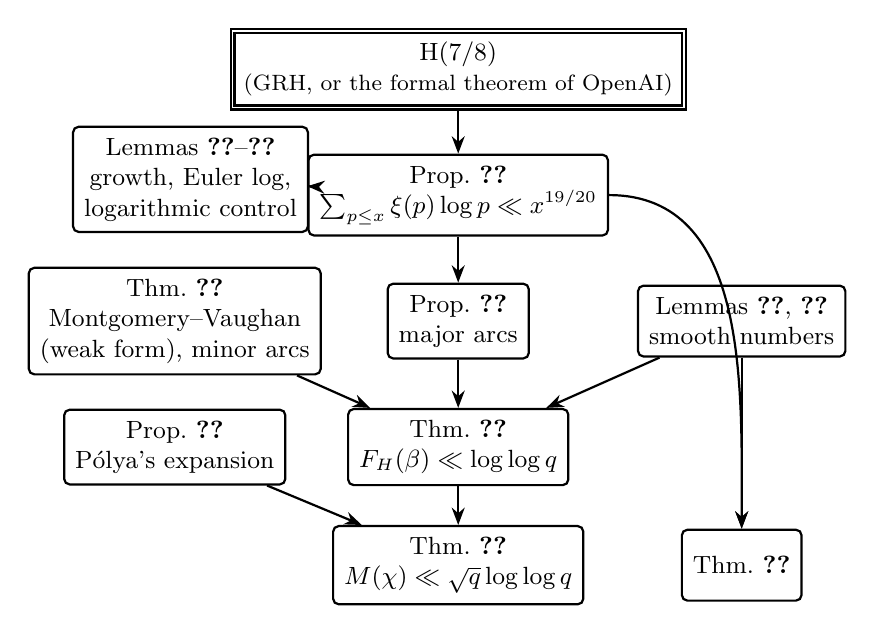
\begin{tikzpicture}[
  box/.style={draw,thick,rounded corners=2pt,align=center,font=\small,inner sep=4pt,minimum height=0.9cm},
  hyp/.style={draw,thick,double,align=center,font=\small,inner sep=4pt,minimum height=0.9cm},
  arr/.style={-{Stealth[length=2.2mm]},thick}]
\node[hyp] (H) at (0,4.2) {$\mathrm H(7/8)$\\ \footnotesize(GRH, or the formal theorem of OpenAI)};
\node[box] (L) at (-3.4,2.8) {Lemmas \ref{lem:growth}--\ref{lem:logcontrol}\\ growth, Euler log,\\ logarithmic control};
\node[box] (P) at (0,2.6) {Prop.~\ref{prop:primesum}\\ $\sum_{p\le x}\xi(p)\log p\ll x^{19/20}$};
\node[box] (Mj) at (0,1.0) {Prop.~\ref{prop:nsmajor}\\ major arcs};
\node[box] (MV) at (-3.6,1.0) {Thm.~\ref{thm:mv}\\ Montgomery--Vaughan\\ (weak form), minor arcs};
\node[box] (Sm) at (3.6,1.0) {Lemmas \ref{lem:smooth}, \ref{lem:psi}\\ smooth numbers};
\node[box] (B) at (0,-0.6) {Thm.~\ref{thm:B}\\ $F_H(\beta)\ll\log\log q$};
\node[box] (Po) at (-3.6,-0.6) {Prop.~\ref{prop:polya}\\ P\'olya's expansion};
\node[box] (T) at (0,-2.1) {Thm.~\ref{thm:main}\\ $M(\chi)\ll\sqrt q\log\log q$};
\node[box] (Tr) at (3.6,-2.1) {Thm.~\ref{thm:range}};
\draw[arr] (H) -- (P); \draw[arr] (L) -- (P); \draw[arr] (P) -- (Mj);
\draw[arr] (Mj) -- (B); \draw[arr] (MV) -- (B); \draw[arr] (Sm) -- (B);
\draw[arr] (B) -- (T); \draw[arr] (Po) -- (T);
\draw[arr] (P) to[out=0,in=90] (Tr); \draw[arr] (Sm) -- (Tr);
\end{tikzpicture}
\caption{The structure of the proof. The double box is the only input about
zeros. Every box is a theorem of the Lean development; the arrows are
logical dependences. The left column (Montgomery--Vaughan and P\'olya's
expansion) is unconditional.}
\label{fig:dep}
\end{figure}

\section{The formal proof}\label{sec:lean}

The Lean~4 sources are in~\cite{repo}, on Lean v4.34.1 and the Mathlib commit
pinned in \texttt{lake-manifest.json}. The hypothesis is the Lean definition
\begin{quote}\small
\texttt{def GRH : Prop :=}
$\forall\,(q:\mathbb N)\ [\texttt{NeZero}\ q]\ (\chi:\texttt{DirichletCharacter}\ \mathbb C\ q)\ (s:\mathbb C),$\\
\hspace*{2em}$1/2<s.\texttt{re}\to\lnot(\chi=1\wedge s=1)\to\texttt{DirichletCharacter.LFunction}\ \chi\ s\ne0$
\end{quote}
and $\mathrm H(7/8)$ is \texttt{PolyaRH.SevenEighths}. The main formal statements are:
\begin{itemize}
\item \texttt{PolyaRH.polya\_vinogradov\_of\_sevenEighths}: Theorem~\ref{thm:main};
\item \texttt{PolyaRH.polya\_vinogradov\_of\_GRH}: Corollary~\ref{cor:grh};
\item \texttt{PolyaRH.polya\_vinogradov}: Corollary~\ref{cor:uncond};
\item \texttt{PolyaRH.character\_sum\_range\_of\_GRH} and \texttt{PolyaRH.character\_sum\_range}: Theorem~\ref{thm:range}.
\end{itemize}
In each, the bound reads $\|\sum_{n\in(0,T]}\chi(n)\|\le C\sqrt q\log\log q$ for all
natural numbers $T$, with $\chi$ primitive modulo $q\ge3$, which is the statement
for real $x$. The command \texttt{\#print axioms} reports only
\texttt{propext}, \texttt{Classical.choice} and \texttt{Quot.sound} for every
one of them, including the unconditional statements, whose proofs pass through
all 2,924 files of OpenAI's library; the output is the file \texttt{axioms.txt}
of the repository. There is no \texttt{sorry}, no new axiom and no
\texttt{native\_decide}.

The Lean library is organised as in the text: \texttt{Vinogradov/PV/Polya} and
\texttt{Gauss} (Section~\ref{sec:polya}); \texttt{MRT}, \texttt{EulerLog},
\texttt{Riesz}, \texttt{ContourShift}, \texttt{Analytic},
\texttt{CharacterSums} and \texttt{PV/PrimeSum} (Section~\ref{sec:analytic});
\texttt{PV/Twist} and \texttt{PV/NonSmooth} (Sections~\ref{sec:major}
and~\ref{sec:nonsmooth}); \texttt{PV/Smooth} (Section~\ref{sec:smooth});
\texttt{MV/*} (Section~\ref{sec:mv}); \texttt{PV/Main} and \texttt{PV/Range}
(Sections~\ref{sec:B} and~\ref{sec:proofs}). The hypothesis enters at one
point only, the lemma \texttt{Vinogradov.zeroFree}, and the formal
dependence of each theorem on it is visible in its type.\footnote{The
hypothesis is carried by a class \texttt{PolyaRH.HalfPlane}, and the theorems
that use it, and only those, take an instance argument of that class. The
statements in \texttt{PolyaRH/Main.lean} discharge it from \texttt{GRH} or from
\texttt{SevenEighths}, and \texttt{PolyaRH/Unconditional.lean} discharges it from
the formal theorem of~\cite{openai}.}

Several files adapt code from other Lean libraries, all under the Apache
License~2.0: the logarithmic control lemma and the Riesz-mean, contour-shift,
growth and Euler-logarithm files from OpenAI's library~\cite{openai}; the
Selberg sieve used for Proposition~\ref{prop:pairs} from
PrimeNumberTheoremAnd~\cite{pnt}, by A.~Mellendijk. The unconditional statements
also compile OpenAI's proof of $\mathrm H(7/8)$, about 2,900 files, together with
the parts of PrimeNumberTheoremAnd and of~\cite{rk} that it imports.

\section*{Acknowledgements}
The author thanks the authors of Mathlib, of PrimeNumberTheoremAnd and of the
OpenAI Lean library, whose code is used and credited in Section~\ref{sec:lean}.

\section*{Data availability}
All Lean sources, the build instructions and the output of \texttt{\#print
axioms} are in the public repository~\cite{repo}.

\bibliographystyle{amsplain}
\bibliography{refs}
\end{document}
